% =====================================================================================================
%  Early exits for weight-memory fault detection and tolerance: calibrated logit bands against SDC
%  Source of every number: /home1/jtt/early_exit_final/stage2_paper/results/paper/paper_tables.md
%  (tables T2-T14, R) and results/offline/final/runs_exponent.csv.gz (per-k data of Fig. 2).
%  All tables are inline (booktabs). Plots are PNGs in figures/, made by make_figures.py
%  (run: ../.venv/bin/python make_figures.py figures).
%  Lines marked "TODO" need the authors' input (author list, venue).
% =====================================================================================================
\documentclass[10pt,a4paper]{article}

\usepackage[utf8]{inputenc}
\usepackage[T1]{fontenc}
\usepackage{lmodern}
\usepackage[margin=2.2cm]{geometry}
\usepackage{amsmath,amssymb}
\usepackage{booktabs}
\usepackage{multirow}
\usepackage{array}
\usepackage{xcolor}
\usepackage{caption}
\usepackage{float}      % [H]: keep every table/figure exactly where its explanation is
\usepackage{adjustbox}  % shrink a table only if it is wider than the text
\usepackage{tikz}
\usetikzlibrary{positioning,arrows.meta,fit}
\usepackage{graphicx}
\graphicspath{{figures/}}
\usepackage{hyperref}

\newcommand{\meth}[1]{\texttt{#1}}
\newcommand{\ours}{\meth{margin\_band}}
\definecolor{cplain}{HTML}{6B6B6B}
\definecolor{csdn}{HTML}{E08A1E}
\definecolor{cmend}{HTML}{C0392B}
\definecolor{cenergy}{HTML}{8E44AD}
\definecolor{cours}{HTML}{1F6FB2}
\definecolor{cmax}{HTML}{27AE60}

\title{Early Exits for Weight-Memory Fault Detection and Tolerance:\\
Calibrated Logit Bands Against Silent Data Corruption in CNNs}
\author{TODO: authors and affiliations}
\date{}

\begin{document}
\maketitle

% -----------------------------------------------------------------------------------------------------
\begin{abstract}
Bit flips in the weight memory of a deep neural network (DNN) can turn correct predictions into wrong
ones without any warning, a \emph{silent data corruption} (SDC). Early-exit networks attach small
classifiers to intermediate layers to save computation on easy inputs. We show that the same exits can
detect weight-memory faults, and partly tolerate them, at almost no extra cost. The key observation is that the most damaging faults,
flips of high exponent bits in FP32 weights, make the network \emph{over-confident}: logits become
abnormally large. Confidence-based detectors, including the recent early-exit method MENDNet, flag only
\emph{low} confidence and therefore miss these faults. We calibrate, on clean validation data only, a
two-sided band on the maximum logit at every exit and at the final classifier, with a false-alarm budget
$\alpha$. Inputs whose final logits leave the band are flagged instead of being answered silently. The
check needs only comparators and one subtraction per exit. The exit positions and head architectures are
chosen by multi-objective architecture search. Flagged inputs receive a fallback answer from an exit
whose output is still in its band. On VGG16-BN / CIFAR-10, with $3{,}200$ fault-injection runs of
$10{,}000$ test images each, each run flipping one random exponent bit in each of $1$ to $8$ random
weights, the method lowers the SDC rate from $13.4\,\%$ (plain network) and
$7.35\,\%$ (MENDNet) to $0.22\,\%$, detects $93.1\,\%$ of harmful fault runs with a $0.08\,\%$ run-level
false-positive rate, and still saves $60.5\,\%$ of the FLOPs, at a cost of $1.1$ points of clean
accuracy and a $0.95\,\%$ clean false-alarm rate. Under faults, accuracy rises from $80.0\,\%$ (plain
network) to $87.4\,\%$ with fallback. Real early stopping makes batch-1 inference
$3.3\times$ faster on CPU and $1.4\times$ faster on an A100 GPU.
\end{abstract}

% -----------------------------------------------------------------------------------------------------
\section{Introduction}

DNN accelerators keep millions of weights in on-chip and off-chip memory. Radiation, ageing, voltage
scaling and manufacturing defects cause bit flips in these memories. A single flip of a high exponent bit
of an FP32 weight can change its value by many orders of magnitude, and the network then gives wrong
answers with no indication that anything is wrong.

\paragraph{Silent data corruption.} For an input $x$ that the fault-free system classifies correctly, a
fault causes a \emph{silent data corruption} (SDC) if the faulty system returns a \emph{wrong} label for $x$
and raises \emph{no} flag. If the faulty system raises a flag instead, the error is \emph{detected}; if it
still returns the correct label, the fault is \emph{masked}. SDCs are the main concern in safety-critical
use, because a detected error can be handled (retry, reload, fall back to a safe action) while a silent one
cannot. The SDC rate used throughout this paper is defined formally in Section~\ref{sec:setup}.

Classical protection (ECC, modular redundancy, re-execution) costs area, energy or latency. Early-exit
networks~\cite{branchynet,sdn} already add small classifiers (\emph{exits}) at intermediate layers so that
easy inputs stop early and save computation. Their outputs are a cheap, independent view of the input at
several depths. This paper asks whether these exits can serve as a fault detector at the same time, with
no extra network and almost no extra hardware.

\paragraph{Observation.} Detectors based on confidence or energy~\cite{msp,energy} and the recent
early-exit fault detector MENDNet~\cite{mendnet} flag an input when the network is \emph{uncertain}.
Exponent-bit faults do the opposite: they inflate the logits, so the corrupted network looks
\emph{more} confident than usual (Section~\ref{sec:ablation}). A detector that checks only the low side
misses almost all of these faults.

\paragraph{Contributions.} The individual building blocks of our rule are known: early exit on the margin
between the two largest logits~\cite{bigLittle}, the maximum logit as a confidence score~\cite{maxlogit}, and
value-range checks or clipping against hardware faults~\cite{li2017,ranger,ftclipact}. Our contributions are their
combination for early-exit networks under weight-memory faults, the analysis of why it works, the search of the
exit architecture, and the evaluation. Compared with MENDNet~\cite{mendnet}, the closest work:
\begin{enumerate}
  \item \textbf{Finding: weight-memory faults make early-exit networks over-confident.} We show that the most
        damaging faults (high exponent bits) inflate the logits, so uncertainty-based detectors, including
        MENDNet's energy criterion, miss them (run-level TPR below $5\,\%$), while an upper bound on the maximum
        logit catches them (ablation, Table~\ref{tab:ablation}).
  \item \textbf{Range check at the exits, calibrated on clean data only.} We apply a two-sided band on the maximum
        logit at every exit and at the final classifier of an early-exit network, set from clean validation data
        with an explicit false-alarm budget $\alpha$. MENDNet tunes its thresholds on fault-injected data; our rule
        needs no fault data. The margin decides early exit, the band decides acceptance, so one set of exits saves
        $60.5\,\%$ of the FLOPs and lowers SDC by $\approx 60\times$. The decision needs only a top-2 comparator
        tree, one subtraction and three comparisons per exit (Table~\ref{tab:ops}).
  \item \textbf{Exit architecture by multi-objective search, validated step by step.} MENDNet uses fixed exits.
        We search exit positions, head architectures and the rule (accuracy, expected FLOPs, head parameters),
        compare TPE, NSGA-II, random search, restricted spaces and fault-aware objectives, and validate the proxy,
        the fault probe and the final pick (Section~\ref{sec:nasres}).
  \item \textbf{A fair, reproducible evaluation.} All methods are evaluated offline on the \emph{same} stored
        faulty logits (3{,}200 runs $\times$ 10{,}000 images), against six baselines including MENDNet with both
        clean and faulty-data calibration, under three fault models (FP32 exponent, MENDNet's sign-flip model,
        INT8), with run-level detection statistics and measured latency.
\end{enumerate}

% -----------------------------------------------------------------------------------------------------
\section{Related work}

\paragraph{Early-exit networks.} BranchyNet~\cite{branchynet} and Shallow-Deep Networks (SDN)~\cite{sdn}
attach classifiers to intermediate layers and stop when the softmax confidence is high enough. They target
efficiency and overthinking, not faults.

\paragraph{Fault resilience of DNNs.} Fault-injection studies~\cite{li2017,ares} show that a few flips of
high exponent bits dominate the damage in floating-point DNNs, and that reduced-precision integer formats
are more robust. Protection ranges from ECC and redundancy to software techniques.

\paragraph{Range checks and range restriction.} Value ranges are an established defence against hardware faults.
Li~\emph{et al.}~\cite{li2017} propose symptom-based error detectors that flag activation values outside ranges
profiled on fault-free runs. Ranger~\cite{ranger} clips the outputs of selected layers to profiled bounds and
turns critical soft errors into benign ones. FT-ClipAct~\cite{ftclipact} replaces unbounded activation functions
by clipped ones to tolerate permanent faults in weight memory, also on VGG-16 / CIFAR-10. Our band is a range check
of the same kind; the difference is \emph{where} it is applied (on the 10 logits of each exit and of the final
classifier instead of on internal activations), that it serves as an early-exit acceptance test as well as a
detector, and that it is calibrated for an explicit false-alarm budget. Range checks on internal activations are
complementary and could be combined with it.

\paragraph{Confidence-based detection.} The maximum softmax probability~\cite{msp} and the energy
score~\cite{energy} are standard detectors of abnormal inputs; the maximum logit~\cite{maxlogit} is a further
strong score. They are used to flag \emph{low} confidence. Early exit on the margin between the two largest
scores goes back to big/little networks~\cite{bigLittle}.

\paragraph{MENDNet~\cite{mendnet}.} MENDNet uses the exits of an early-exit network to detect and
mitigate weight faults: an input is flagged as faulty when no exit reaches a negative-energy threshold
$\tau$, and the label of the least uncertain exit is returned. Its thresholds $(\gamma,\tau)$ are tuned on
fault-injected data. We re-implement its Algorithm~1 and evaluate it with both a clean calibration and
its own faulty-data calibration (on validation faults only).

% -----------------------------------------------------------------------------------------------------
\section{Problem definition: fault model, detection and tolerance}\label{sec:problem}

This section states precisely which faults we consider, what we mean by fault detection and by fault
tolerance, and how each is measured. The numbers quoted here are proved in Section~\ref{sec:results}.

\subsection{Fault model: weight-memory bit flips}\label{sec:faultmodel}

We consider faults in the \emph{memory that stores the weights} of the network (on-chip SRAM or off-chip
DRAM). Such faults are caused, for example, by radiation (soft errors), ageing, reduced supply voltage or
manufacturing defects. A fault is a single flipped bit in a stored weight; the computation itself is
assumed to be correct. Table~\ref{tab:faultmodel} lists every property of the main fault model.

\begin{table}[H]
\centering\small
\caption{Main fault model (FP32 exponent faults in weight memory).}
\label{tab:faultmodel}
\begin{adjustbox}{max width=\linewidth}
\begin{tabular}{@{}p{0.24\linewidth}p{0.70\linewidth}@{}}
\toprule
Property & Choice in this paper \\
\midrule
What is faulted        & Stored weights of all convolution and fully connected layers (backbone and exit heads). \\
What is not faulted    & Activations, arithmetic units, control logic, biases and batch-normalisation parameters. \\
Which bit              & One exponent bit of an FP32 weight, chosen uniformly from bits 23--30. Sign and mantissa
                         bits are not faulted in the main model. \\
How many               & $k\in\{1,\dots,8\}$ faulty weights per run, all different, with one flipped bit each
                         (a run never flips several bits of one weight). \\
Which weights          & Drawn uniformly at random from one location per run: G1 (backbone before the first exit),
                         G2 (between the first and the last exit), G3 (after the last exit, plus the classifier) or
                         HEADS (the exit heads). \\
Duration               & Persistent: the faulty weights stay in memory for the whole run (all 10{,}000 test images),
                         as a memory fault does until the weights are reloaded. \\
Excluded faults        & Faults that make any weight or output infinite or NaN are redrawn, because such outputs are
                         trivially detectable; all reported errors come from finite, plausible-looking outputs. \\
Scale                  & 100 runs per (location, $k$): $4\times8\times100 = 3{,}200$ runs on 10{,}000 test images,
                         32 million faulty inferences per method. \\
Additional models      & (a) MENDNet's model: sign-bit flips of 10--50\,\% of one layer group's weights;
                         (b) simulated weight-only INT8: one flipped bit in each of $k$ INT8 weight codes. \\
\bottomrule
\end{tabular}
\end{adjustbox}
\end{table}

For one fault-free input $x$ with true label $y$, a fault has exactly one of four outcomes (Table~\ref{tab:outcomes}):

\begin{table}[H]
\centering\small
\caption{Outcome of a fault for one input that the fault-free system answers correctly.}
\label{tab:outcomes}
\begin{adjustbox}{max width=\linewidth}
\begin{tabular}{@{}lll@{}}
\toprule
Outcome & Faulty system output & Meaning \\
\midrule
Masked                          & correct label, no flag  & the fault has no effect on this input (tolerated) \\
\textbf{Silent data corruption} & wrong label, no flag    & \textbf{undetected error: the case we must prevent} \\
Detected                        & flag raised             & the error is reported and can be handled \\
Detected and recovered          & flag raised, fallback label correct & the error is reported \emph{and} the answer is still right \\
\bottomrule
\end{tabular}
\end{adjustbox}
\end{table}

\subsection{Fault detection}\label{sec:defdetect}

\emph{Fault detection} means that the system itself notices that its output is unreliable and raises a
\emph{flag} instead of silently returning a wrong label. In our method an input is flagged when it reaches the
final classifier without being accepted, i.e.\ when the final maximum logit lies outside its calibrated band
(Eq.~\eqref{eq:final}). Detection is measured at two levels:
\begin{itemize}
  \item \textbf{per image:} the SDC rate (wrong and not flagged) and the detection ratio (flagged among all
        images the fault would have corrupted);
  \item \textbf{per run:} whether the flag count of a run is significantly above the clean false-alarm rate
        (binomial test), i.e.\ whether the system can tell that its memory is faulty; reported as TPR on harmful
        runs, FPR on harmless runs, and the number of images needed until detection.
\end{itemize}
\textbf{Achieved:} yes. The SDC rate falls from $13.4\,\%$ (plain network) to $0.22\,\%$; $95.9\,\%$ of the
would-be corruptions are flagged; $93.1\,\%$ of harmful fault runs are detected (FPR $0.08\,\%$), after a median of
200 images (Table~\ref{tab:main}).

\subsection{Fault tolerance}\label{sec:deftol}

\emph{Fault tolerance} means that the system still returns \emph{correct} answers while the fault is present.
We measure it as the accuracy on all 10{,}000 test images under faults, and as the share of the accuracy lost by
the plain network that is recovered. Our method provides tolerance by two mechanisms, and does \emph{not} repair
the faulty weights:
\begin{enumerate}
  \item \textbf{Early exit:} an input that leaves at an exit placed before the faulty layer never uses the faulty
        weight, so the fault is masked for that input.
  \item \textbf{Fallback:} a flagged input receives the label of the most confident exit whose output is still in
        its band (Section~\ref{sec:fallback}).
\end{enumerate}
\textbf{Achieved:} partly. Under exponent faults the plain network drops from $92.3\,\%$ to $80.0\,\%$; with our
method the accuracy is $87.4\,\%$, i.e.\ $60\,\%$ of the lost accuracy is recovered (Table~\ref{tab:tolerance}).
Most of this comes from early exit; the band and the fallback add about one point over early exit alone. Full
recovery would require repairing the memory (reloading the weights) once a faulty run is detected, which our
run-level detection enables but which is not evaluated here.

\subsection{Questions answered in this paper}

Table~\ref{tab:questions} lists the questions this paper answers, the short answer, and where the evidence is.

\begin{table}[H]
\centering\small
\caption{Research questions and where they are answered.}
\label{tab:questions}
\begin{adjustbox}{max width=\linewidth}
\begin{tabular}{@{}p{0.40\linewidth}p{0.36\linewidth}p{0.17\linewidth}@{}}
\toprule
Question & Short answer & Where \\
\midrule
Which faults are considered?                           & Weight-memory bit flips, 1--8 random weights, one exponent bit each & Sec.~\ref{sec:faultmodel} \\
Can early exits detect weight-memory faults?           & Yes: SDC $13.4\to0.22\,\%$, run TPR $93.1\,\%$ & Tab.~\ref{tab:main} \\
Why do existing detectors miss them?                   & Faults make the network over-confident; only the upper side of the band catches them & Tab.~\ref{tab:ablation} \\
Is fault tolerance achieved?                           & Partly: accuracy $80.0\to87.4\,\%$, $60\,\%$ of the loss recovered & Tab.~\ref{tab:tolerance} \\
Where and which bits are dangerous?                    & G1 (before the first exit); exponent bit 30 & Tab.~\ref{tab:loc}, \ref{tab:bit} \\
Does it work for other fault models?                   & INT8: faults nearly harmless; MENDNet model: mixed & Tab.~\ref{tab:int8}--\ref{tab:mendsdc} \\
What does it cost?                                     & $-1.1$ points clean accuracy, $0.95\,\%$ false alarms; comparators only & Tab.~\ref{tab:main}, \ref{tab:ops} \\
Is the compute saving real?                            & Yes: $60.5\,\%$ FLOPs, $3.3\times$ CPU, $1.4\times$ GPU & Tab.~\ref{tab:latency} \\
Is every step of the exit search justified?            & Yes: strategy, proxy, fault probe, designs, full training & Sec.~\ref{sec:nasres} \\
\bottomrule
\end{tabular}
\end{adjustbox}
\end{table}

% -----------------------------------------------------------------------------------------------------
\section{Method}\label{sec:method}

\subsection{Early-exit model}

The backbone is a VGG16-BN $f$ with feature modules $f_0,\dots,f_{43}$ (13 convolutions with batch
normalisation and ReLU, 5 max-pools) followed by global average pooling and the classifier
$512\!\to\!512\!\to\!10$. The backbone is trained once and then \emph{frozen}; exits never change its
weights. An exit $k\in\{1,\dots,K\}$ is a small head $h_k$ attached after module $p_k$:
\[
  z_k(x) = h_k\big(f_{p_k}\circ\dots\circ f_0(x)\big)\in\mathbb{R}^{10},\qquad
  z_{K+1}(x) = \text{final classifier logits}.
\]
Each head is \texttt{[conv block]}$^{n}$ $\to$ adaptive average pooling to $q\times q$ $\to$ optional
hidden FC layer $\to$ FC to 10 classes. A conv block is either a standard $3\times3$ convolution or a
depthwise-separable one, with output channels $C\cdot r$, followed by BN and ReLU.
Search space per exit: $n\in\{0,1,2\}$, conv type $\in\{\text{std},\text{dw-sep}\}$,
$r\in\{1/2,1/4,1/8\}$, $q\in\{1,2,4\}$, hidden width $\in\{0,64,128,256\}$; position $p_k$ from 17
candidates; $K\in\{1,2,3\}$. Heads are trained on the frozen backbone with knowledge distillation from the
final classifier (temperature 3, weight 0.3), Adam, learning rate $10^{-3}$, weight decay $10^{-4}$,
cosine schedule, 60 epochs.

Figure~\ref{fig:arch} shows the selected model: exits after modules 13, 16 and 26.

\begin{figure}[H]
\centering
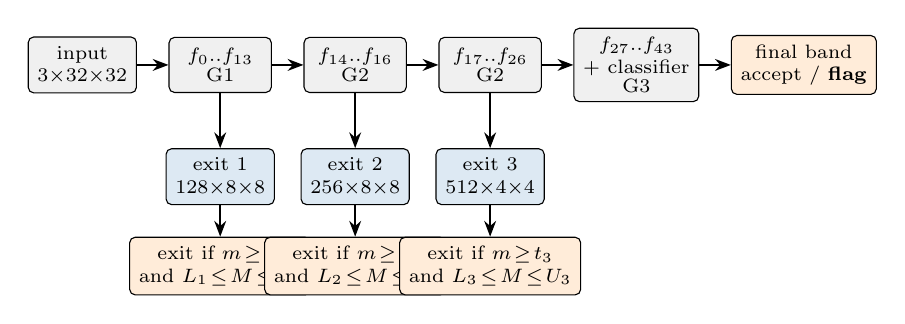
\begin{tikzpicture}[
  blk/.style={draw, rounded corners=2pt, fill=gray!12, minimum height=7mm, minimum width=13mm, font=\scriptsize, align=center},
  head/.style={draw, rounded corners=2pt, fill=cours!15, minimum height=6mm, minimum width=13mm, font=\scriptsize, align=center},
  dec/.style={draw, rounded corners=2pt, fill=orange!15, minimum height=6mm, minimum width=13mm, font=\scriptsize, align=center},
  arr/.style={-{Stealth[length=2mm]}, thick}, node distance=4mm]
  \node[blk] (in) {input\\$3{\times}32{\times}32$};
  \node[blk, right=of in] (b1) {$f_0..f_{13}$\\[-1pt]G1};
  \node[blk, right=of b1] (b2) {$f_{14}..f_{16}$\\[-1pt]G2};
  \node[blk, right=of b2] (b3) {$f_{17}..f_{26}$\\[-1pt]G2};
  \node[blk, right=of b3] (b4) {$f_{27}..f_{43}$\\+ classifier\\[-1pt]G3};
  \node[dec, right=of b4] (d4) {final band\\accept / \textbf{flag}};
  \draw[arr] (in) -- (b1); \draw[arr] (b1) -- (b2); \draw[arr] (b2) -- (b3); \draw[arr] (b3) -- (b4); \draw[arr] (b4) -- (d4);
  \node[head, below=7mm of b1] (h1) {exit 1\\$128{\times}8{\times}8$};
  \node[head, below=7mm of b2] (h2) {exit 2\\$256{\times}8{\times}8$};
  \node[head, below=7mm of b3] (h3) {exit 3\\$512{\times}4{\times}4$};
  \draw[arr] (b1) -- (h1); \draw[arr] (b2) -- (h2); \draw[arr] (b3) -- (h3);
  \node[dec, below=4mm of h1] (d1) {exit if $m\!\ge\!t_1$\\and $L_1\!\le\!M\!\le\!U_1$};
  \node[dec, below=4mm of h2] (d2) {exit if $m\!\ge\!t_2$\\and $L_2\!\le\!M\!\le\!U_2$};
  \node[dec, below=4mm of h3] (d3) {exit if $m\!\ge\!t_3$\\and $L_3\!\le\!M\!\le\!U_3$};
  \draw[arr] (h1) -- (d1); \draw[arr] (h2) -- (d2); \draw[arr] (h3) -- (d3);
\end{tikzpicture}
\caption{Selected early-exit VGG16-BN (exits after modules 13, 16, 26). $m$ = margin (top-1 minus top-2 logit),
$M$ = maximum logit. An input that fails an exit test continues; at the end it is accepted only if its final
maximum logit is inside the final band, otherwise it is \emph{flagged}. G1, G2, G3 and the heads are the
fault-injection locations (G2 merges the two middle segments).}
\label{fig:arch}
\end{figure}

\subsection{Exit and detection rule (\ours)}\label{sec:rule}

For logits $z\in\mathbb{R}^{C}$ let $M(z)=\max_c z_c$ be the maximum logit and
$m(z)=z_{(1)}-z_{(2)}$ the margin between the two largest logits. An input $x$ is processed exit by exit:
\begin{align}
  \text{exit at }k\ (\le K) &\iff z_k\ \text{finite} \;\wedge\; m(z_k)\ge t_k \;\wedge\; L_k\le M(z_k)\le U_k,
  \label{eq:exit}\\
  \text{accept at the final classifier} &\iff z_{K+1}\ \text{finite} \;\wedge\; L_{\mathrm{fin}}\le M(z_{K+1})\le U_{\mathrm{fin}},
  \label{eq:final}
\end{align}
and the input is \textbf{flagged} if it reaches the end without being accepted. The margin threshold $t_k$
decides \emph{whether the exit is confident enough}; the band $[L_k,U_k]$ decides \emph{whether the exit's
output looks normal}. An out-of-band exit does not flag; the input simply continues to deeper exits. The
detection decision is taken once, by the final band.

\paragraph{Why a two-sided band.} Flipping exponent bit $23+i$ multiplies or divides a weight by
$2^{2^i}$. For typical weights ($|w|<2$) bit 30 is 0 and bits 27--29 are 1, so a flip of bit 30 multiplies
the weight by $2^{128}$, while flips of bits 27--29 divide it by $2^{16}$--$2^{64}$. The inflated weight
dominates its neuron, and the downstream logits grow far beyond their clean range. The network then becomes over-confident, not uncertain. A low-confidence test (MSP,
energy, MENDNet's $\tau$) is satisfied by such inputs; the upper bound $U$ is not.

\subsection{Calibration on clean data only}\label{sec:calib}

All thresholds are set on the clean validation split (5{,}000 images); no fault data is used.
\begin{itemize}
  \item \textbf{Exit bands:} $[L_k,U_k]$ = the $0.1$ and $99.9$ percentiles of $M(z_k)$ on validation.
  \item \textbf{Margin thresholds} (accuracy-aware, exit by exit): among inputs still undecided and inside the
        band, $t_k$ is the smallest value on a percentile grid such that, for $t_k$ and every larger
        threshold, the head's accuracy on the exiting inputs is at most $0.5$ points (\emph{slack}) below
        the final classifier's accuracy on the same inputs (groups smaller than 25 images are ignored).
  \item \textbf{Final band} with false-alarm budget $\alpha$ (default $1\,\%$): among the validation inputs
        reaching the final classifier, $L_{\mathrm{fin}}$ and $U_{\mathrm{fin}}$ cut $\alpha/2$ of the
        \emph{whole} validation set from each tail of $M(z_{K+1})$.
\end{itemize}

\subsection{Mitigation by fallback}\label{sec:fallback}

A flagged input still needs an output in many systems. We return the label of the most confident exit
(largest margin) whose logits are finite and inside its band; the final classifier has no band in this
step. If no exit qualifies, the earliest finite exit is used. This is a light mitigation, similar in spirit
to MENDNet's fallback, and \emph{not} a contribution of this paper; we report it as ``accuracy with
fallback''.

\subsection{Exit-placement search}\label{sec:nas}

Exit positions, head architectures and the rule ($\ours$ or \meth{maxlogit\_band}) are searched with
Optuna~\cite{optuna}. Each trial trains its heads for 8 epochs on cached backbone features (a proxy),
calibrates thresholds on VAL\_CAL (2{,}500 images), and is scored on VAL\_SEL (the other 2{,}500):
maximise accuracy, minimise expected FLOPs, minimise head parameters, subject to accuracy $\ge$ backbone
accuracy $-1$ point. Thresholds are never searched; they are always calibrated. We run TPE~\cite{tpe}
(250 trials) with three sampler seeds and compare it to NSGA-II~\cite{nsga2}, random search,
restricted spaces and fault-aware objectives (Section~\ref{sec:nasres}).

Because the proxy ranking is noisy, the five lowest-FLOPs feasible Pareto points of the three TPE runs, plus
two further candidates, are \emph{fully} trained (60 epochs) and re-scored on VAL\_SEL. The final model is
the lowest-FLOPs candidate with VAL\_SEL accuracy $\ge 91.84\,\%$ (backbone $92.84\,\%$ $-1$); ties go to
fewer head parameters. This gives model \meth{s11\_t229}: exits after modules 13, 16, 26, with $260{,}830$
head parameters ($1.7\,\%$ of the backbone's $14.99$\,M) and $3.67\,\%$ head-FLOP overhead
(Table~\ref{tab:top5}).

% -----------------------------------------------------------------------------------------------------
\section{Experimental setup}\label{sec:setup}

\paragraph{Data and backbone.} CIFAR-10 with a fixed 45k/5k train/validation split and the 10k test set.
VGG16-BN trained with SGD (lr $0.025$, momentum $0.9$, weight decay $5\cdot10^{-4}$, cosine schedule,
100 epochs, random crop and flip); best validation epoch 94. Validation accuracy $92.64\,\%$,
test accuracy $92.27\,\%$, $627.9$ MFLOPs per image (1 MAC = 2 FLOPs).

\paragraph{Methods compared.} Table~\ref{tab:methods}. Every standard rule uses the same calibration
procedure (Section~\ref{sec:calib}) with its own score, so differences come from the signal and the gate,
not from tuning.

\begin{table}[H]
\centering\small
\caption{Methods. ``Exit score'' decides early exit; ``gate'' decides acceptance at the final classifier.
All are calibrated on clean validation data with $\alpha=1\,\%$ (``@1''), except MENDNet-faulty-val.}
\label{tab:methods}
\begin{adjustbox}{max width=\linewidth}
\begin{tabular}{@{}llll@{}}
\toprule
Method & Exit score & Final gate / detection & Role \\
\midrule
\meth{plain\_dnn}            & --- (no exits)          & none                         & baseline: unprotected network \\
\meth{sdn\_msp}              & max softmax             & none                         & baseline: SDN~\cite{sdn} early exit \\
\meth{msp\_low}              & max softmax             & flag low MSP                 & baseline: MSP detector~\cite{msp} \\
\meth{energy\_low}           & $-$energy               & flag low $-$energy           & baseline: energy detector~\cite{energy} \\
\meth{mendnet\_clean}        & MENDNet Alg.~1          & no exit with $-E>\tau$       & baseline: MENDNet, clean calibration \\
\meth{mendnet\_faulty\_val}  & MENDNet Alg.~1          & no exit with $-E>\tau$       & baseline: MENDNet, tuned on faulty val \\
\midrule
\ours\ (\textbf{ours})       & margin                  & max-logit band               & proposed \\
\meth{maxlogit\_band}        & max logit               & max-logit band               & variant \\
\meth{energy\_band}          & $-$energy               & energy band                  & variant \\
\meth{margin\_multiband}     & margin                  & bands on max, min, sum       & variant \\
\meth{margin\_band\_agree}   & margin + agree w/ next  & max-logit band               & variant \\
\bottomrule
\end{tabular}
\end{adjustbox}
\end{table}

\paragraph{Fault models} (summarised in Table~\ref{tab:faultmodel}).
\begin{enumerate}
  \item \textbf{FP32 exponent faults (main).} $k\in\{1,\dots,8\}$ distinct weights of convolution and
        linear layers are drawn uniformly within one location (G1: modules before exit 1; G2: between
        the first and last exit; G3: after the last exit plus the classifier; HEADS: the exit heads), and
        one exponent bit of each, chosen uniformly from bits 23--30, is flipped. A run with $k$ faults therefore
        has exactly $k$ single-bit flips in $k$ different weights (never several flips in one weight); the
        sign and mantissa bits are not faulted. Faults are persistent: they stay in memory for all
        10{,}000 test images of the run. Faults that make any weight or logit
        non-finite are rejected and redrawn, so all reported SDCs come from finite, plausible-looking
        outputs. 100 runs per (location, $k$): 3{,}200 runs on the full 10k test set.
  \item \textbf{MENDNet's fault model}~\cite{mendnet}: sign-bit flips of a fraction FR $\in\{10,30,50\}\,\%$
        of the weights of one group (FP1 final classifier, FP2 exit-2 head, FP3 first conv after exit 1,
        FP4 first conv), 10 runs each.
  \item \textbf{INT8 weight faults:} simulated weight-only INT8 (symmetric per-tensor, codes in
        $[-127,127]$, activations in FP32); one of the 8 bits of $k$ codes is flipped. Clean test
        accuracy after quantisation is $92.26\,\%$.
\end{enumerate}
Each campaign stores the logits of every exit for every image and run. All methods are then evaluated
offline on identical faults. After each run all weights are restored and checked bit-identical.
MENDNet-faulty-val is tuned on a separate validation campaign (10 runs per setting, different seeds);
test faults are never used for tuning.

\paragraph{Metrics.} For method $m$, let $S_m$ be the clean test images that $m$ answers correctly
without a flag.
\begin{itemize}
  \item \textbf{SDC rate}: fraction of $S_m$ that is accepted with a wrong label under the fault.
  \item \textbf{Flag rate}: fraction of $S_m$ flagged under the fault; \textbf{detection ratio} =
        flagged / (flagged + SDC) on $S_m$; \textbf{precision}: flagged images whose logits actually
        changed / all flagged.
  \item \textbf{Clean FAR}: flag rate on clean test data; \textbf{FLOPs saved}: $1-$ expected FLOPs / plain
        VGG16 FLOPs.
  \item \textbf{Run-level detection}: a run is detected if its flag count is significant against the
        clean FAR (binomial test, $p<0.01$). TPR is measured on \emph{critical} runs (the unprotected
        early-exit model loses $\ge 1$ point), FPR on \emph{benign} runs ($<0.1$ point).
        \textbf{Detection latency}: median number of images (windows of 100) until the first significant
        window.
  \item \textbf{Accuracy under faults} on all test images, with flagged images counted as wrong, and
        \textbf{with fallback} (Section~\ref{sec:fallback}).
\end{itemize}

% -----------------------------------------------------------------------------------------------------
\section{Results}\label{sec:results}

\subsection{Main comparison}

\begin{table}[H]
\centering\small
\setlength{\tabcolsep}{3.6pt}
\caption{Method comparison on the final model, FP32 exponent faults, all locations, $k=1..8$
(3{,}200 runs $\times$ 10{,}000 test images). Clean acc., FAR and FLOPs saved on clean test data; all other
columns under faults. TPR/FPR: run-level, binomial test. Latency: median images to detection.}
\label{tab:main}
\begin{adjustbox}{max width=\linewidth}
\begin{tabular}{@{}lrrrrrrrrrr@{}}
\toprule
 & \multicolumn{3}{c}{Clean} & \multicolumn{7}{c}{Under exponent faults} \\
\cmidrule(lr){2-4}\cmidrule(l){5-11}
Method & Acc. & FAR & Saved & \textbf{SDC} & Flag & Det.\ ratio & TPR & FPR & Latency & Acc.\ / fallback \\
 & \% & \% & \% & \% & \% & \% & \% & \% & images & \% \\
\midrule
\meth{plain\_dnn}          & 92.3 & 0    & 0$^\dagger$ & 13.4  & 0      & 0    & 0    & 0     & ---   & 80.0 / 80.0 \\
\meth{sdn\_msp}            & 91.8 & 0    & 60.0 & 6.30  & 0      & 0    & 0    & 0     & ---   & 86.2 / 86.2 \\
\meth{msp\_low}            & 91.4 & 0.96 & 60.0 & 6.23  & 0.036  & 0.57 & 3.5  & 0.08  & 3400  & 85.9 / 86.2 \\
\meth{energy\_low}         & 90.9 & 1.16 & 55.3 & 7.14  & 0.024  & 0.34 & 4.8  & 0.08  & 2900  & 84.6 / 84.9 \\
\meth{mendnet\_clean}      & 91.6 & 1.12 & 54.3 & 7.35  & 0.025  & 0.34 & 4.8  & 0.08  & 2900  & 85.0 / 85.3 \\
\meth{mendnet\_faulty\_val}& 91.2 & 0    & 61.2 & 6.12  & 0      & 0    & 0    & 0     & ---   & 85.8 / 85.8 \\
\midrule
\ours\ (\textbf{ours})     & 91.2 & 0.95 & 60.5 & \textbf{0.223} & 5.25 & 95.9 & 93.1 & 0.08 & 200 & \textbf{86.4 / 87.4} \\
\meth{maxlogit\_band}      & 90.9 & 0.99 & 55.5 & 0.181 & 5.81   & 97.0 & 92.5 & 0.51  & 100   & 85.6 / 86.7 \\
\meth{energy\_band}        & 90.8 & 0.96 & 55.3 & 0.181 & 5.91   & 97.0 & 85.6 & 0.34  & 100   & 85.4 / 86.5 \\
\meth{margin\_multiband}   & 91.2 & 0.99 & 60.4 & 0.212 & 5.28   & 96.1 & 93.8 & 0.25  & 200   & 86.3 / 87.4 \\
\meth{margin\_band\_agree} & 91.3 & 1.17 & 48.9 & 0.174 & 6.78   & 97.5 & 97.1 & 0.34  & 100   & 85.1 / 86.6 \\
\bottomrule
\end{tabular}
\end{adjustbox}\\[2pt]
{\footnotesize $^\dagger$The plain network executes no heads; the evaluation pipeline reports $-3.67\,\%$ because it
charges the head FLOPs to every method.}
\end{table}

Table~\ref{tab:main} gives the central result. The unprotected network silently corrupts $13.4\,\%$ of
its correct answers. Early exit alone (\meth{sdn\_msp}) halves this, because images that leave before the
faulty layer are unaffected, but it detects nothing. Low-confidence detectors and MENDNet flag almost no
corrupted images (detection ratio below $1\,\%$, run-level TPR below $5\,\%$); tuned on faulty
validation data, MENDNet's threshold drops to zero flags. All two-sided band rules lower the SDC rate to
about $0.2\,\%$, and flag $96$--$97.5\,\%$ of the would-be corruptions. \ours\ gives the best trade-off: the
same FLOP saving as SDN ($60.5\,\%$), SDC $0.223\,\%$ ($60\times$ below the plain network, $33\times$ below
MENDNet), run-level TPR $93.1\,\%$ at $0.08\,\%$ FPR, and detection after a median of 200 images.

In accuracy under faults the gain is small ($86.4\,\%$, $87.4\,\%$ with fallback, against $86.2\,\%$
for SDN): the band does not repair the network, it turns silent errors into flagged ones.
Figure~\ref{fig:sdck} shows the same comparison for each number of faulty weights $k$.

\begin{figure}[H]
\centering
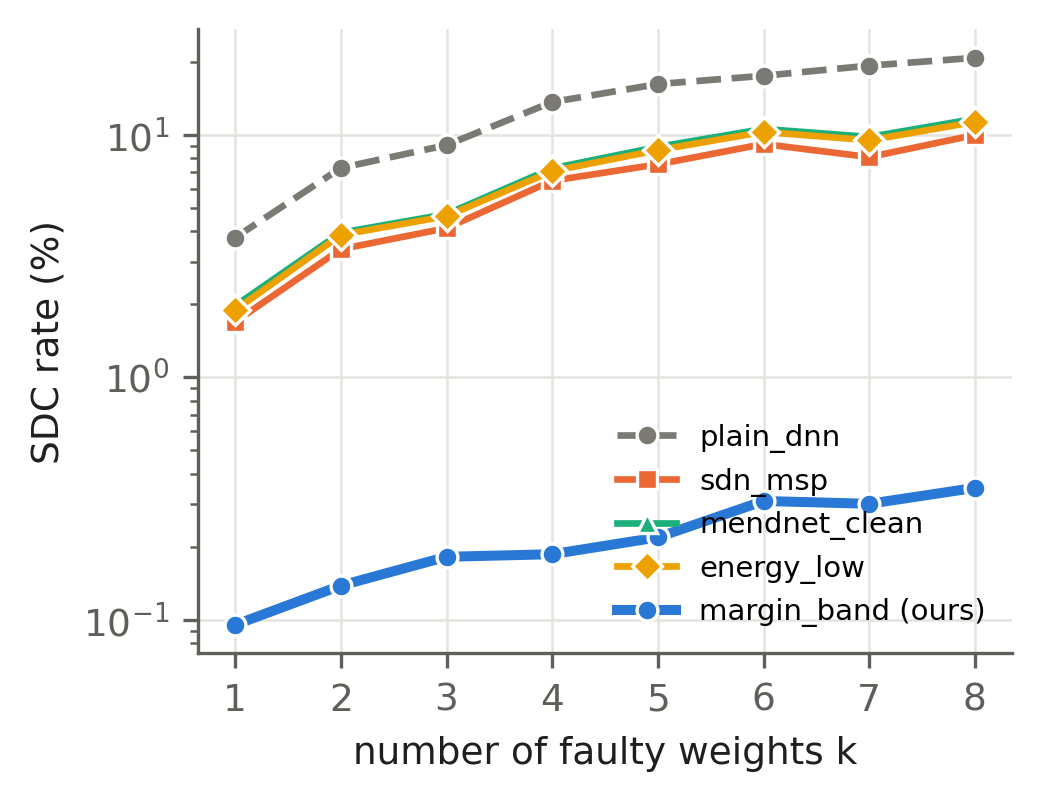
\includegraphics[width=0.48\linewidth]{sdc_vs_k.png}\hfill
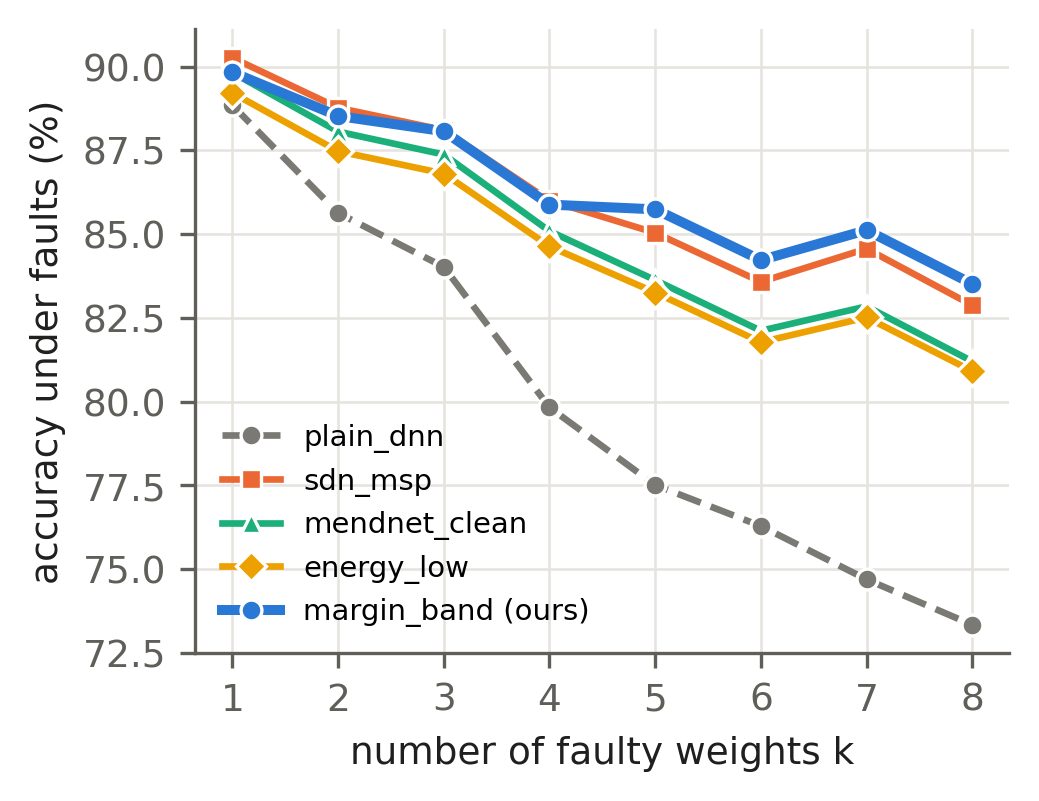
\includegraphics[width=0.48\linewidth]{acc_vs_k.png}
\caption{FP32 exponent faults on the final model, mean over locations and 100 runs per point. Left: SDC rate
(log scale). The band keeps SDC below $0.35\,\%$ even at $k=8$, while all one-sided methods follow the plain
network. Right: accuracy on all test images (flagged = wrong).}
\label{fig:sdck}
\end{figure}

\subsection{Is fault detection achieved? Is fault tolerance achieved?}\label{sec:dettol}

\begin{table}[H]
\centering\small
\caption{Detection and tolerance under FP32 exponent faults (final model). Recovered = share of the plain network's
fault-induced accuracy loss ($92.3-80.0=12.3$ points) that the method wins back: $(\text{acc}-80.0)/12.3$.}
\label{tab:tolerance}
\begin{adjustbox}{max width=\linewidth}
\begin{tabular}{@{}lrrrrrr@{}}
\toprule
 & \multicolumn{3}{c}{Detection} & \multicolumn{3}{c}{Tolerance} \\
\cmidrule(lr){2-4}\cmidrule(l){5-7}
Method & SDC (\%) & Det.\ ratio (\%) & Run TPR (\%) & Acc.\ under faults (\%) & with fallback (\%) & Recovered (\%) \\
\midrule
\meth{plain\_dnn}      & 13.4  & 0    & 0    & 80.0 & 80.0 & 0 \\
\meth{sdn\_msp}        & 6.30  & 0    & 0    & 86.2 & 86.2 & 50 \\
\meth{energy\_low}     & 7.14  & 0.34 & 4.8  & 84.6 & 84.9 & 40 \\
\meth{mendnet\_clean}  & 7.35  & 0.34 & 4.8  & 85.0 & 85.3 & 43 \\
\meth{mendnet\_faulty\_val} & 6.12 & 0 & 0  & 85.8 & 85.8 & 47 \\
\midrule
\ours\ (\textbf{ours}) & \textbf{0.223} & \textbf{95.9} & \textbf{93.1} & \textbf{86.4} & \textbf{87.4} & \textbf{60} \\
\bottomrule
\end{tabular}
\end{adjustbox}
\end{table}

\textbf{Detection: yes.} Table~\ref{tab:tolerance} separates the two properties. Only the band rules detect the
faults: \ours\ flags $95.9\,\%$ of the would-be corruptions and detects $93.1\,\%$ of harmful runs, whereas the
baselines detect below $5\,\%$ of harmful runs or nothing at all.

\textbf{Tolerance: partly.} With fallback, \ours\ keeps $87.4\,\%$ accuracy under faults and recovers $60\,\%$ of the
accuracy the plain network loses, the best of all methods. Early exit alone already recovers $50\,\%$
(\meth{sdn\_msp}), so the band and the fallback add 10 points of recovery on top. The remaining loss is not
recovered because the faulty weights are not repaired; since the faulty run is detected within about 200 images,
reloading the weights at that moment is the natural next step towards full tolerance (Section~\ref{sec:disc}).

\subsection{Where faults are caught}

\begin{table}[H]
\centering\small
\caption{SDC and flag rate (\%) per fault location (final model, exponent faults, $k=1..8$).}
\label{tab:loc}
\begin{adjustbox}{max width=\linewidth}
\begin{tabular}{@{}lrrrrrrrr@{}}
\toprule
 & \multicolumn{4}{c}{SDC rate} & \multicolumn{4}{c}{Flag rate} \\
\cmidrule(lr){2-5}\cmidrule(l){6-9}
Method & G1 & G2 & G3 & HEADS & G1 & G2 & G3 & HEADS \\
\midrule
\meth{plain\_dnn}          & 15.6  & 21.8   & 16.4    & 0      & 0      & 0      & 0       & 0 \\
\meth{sdn\_msp}            & 16.0  & 2.65   & 0.736   & 5.79   & 0      & 0      & 0       & 0 \\
\meth{msp\_low}            & 16.0  & 2.55   & 0.671   & 5.74   & 0.100  & 0.036  & 0.004   & 0.004 \\
\meth{energy\_low}         & 15.9  & 4.31   & 1.01    & 7.37   & 0.070  & 0.023  & 0.003   & 0.0003 \\
\meth{mendnet\_clean}      & 15.8  & 4.98   & 0.952   & 7.62   & 0.072  & 0.025  & 0.004   & 0.0008 \\
\meth{mendnet\_faulty\_val}& 16.1  & 2.64   & 0.393   & 5.38   & 0      & 0      & 0       & 0 \\
\midrule
\ours\ (\textbf{ours})     & 0.621 & 0.0893 & 0.0019  & 0.179  & 17.2   & 2.71   & 0.542   & 0.551 \\
\meth{maxlogit\_band}      & 0.537 & 0.0912 & 0.0027  & 0.0935 & 17.2   & 4.31   & 1.23    & 0.482 \\
\meth{energy\_band}        & 0.535 & 0.0978 & 0.0028  & 0.0904 & 17.2   & 4.63   & 1.08    & 0.728 \\
\meth{margin\_multiband}   & 0.589 & 0.0872 & 0.0019  & 0.168  & 17.2   & 2.74   & 0.544   & 0.585 \\
\meth{margin\_band\_agree} & 0.460 & 0.0651 & 0.0156  & 0.155  & 17.2   & 5.87   & 2.11    & 1.88 \\
\bottomrule
\end{tabular}
\end{adjustbox}
\end{table}

Table~\ref{tab:loc} shows that faults in G1, before the first exit, are the hardest: every exit sees
corrupted features, so early exit gives no protection ($\approx 16\,\%$ SDC for every one-sided method).
The band still catches them, because the corruption propagates into abnormal logits at every depth:
SDC falls from $\approx16\,\%$ to $0.62\,\%$, and $17.2\,\%$ of the images are flagged. Faults in G2 and G3
are partly avoided by early exit and almost fully caught by the band. Faults in the heads leave the backbone intact; the exit bands keep most inputs with abnormal head outputs
from leaving early (SDC $5.79\,\%\to0.18\,\%$ against SDN).

\subsection{Which bits matter}

\begin{table}[H]
\centering\small
\caption{SDC rate (\%) for a single fault ($k=1$) by flipped exponent bit (final model).}
\label{tab:bit}
\begin{adjustbox}{max width=\linewidth}
\begin{tabular}{@{}lrrrrrrrr@{}}
\toprule
Method & bit 23 & 24 & 25 & 26 & 27 & 28 & 29 & 30 \\
\midrule
\meth{plain\_dnn}          & 0.0008 & 0.0018 & 0.026 & 0.240 & 0.0002 & 0      & 0      & 36.4 \\
\meth{sdn\_msp}            & 0.0017 & 0.0048 & 0.058 & 0.588 & 0.0009 & 0.0014 & 0.0010 & 15.6 \\
\meth{mendnet\_clean}      & 0.0021 & 0.0058 & 0.035 & 0.493 & 0.0016 & 0.0021 & 0.0010 & 18.5 \\
\meth{mendnet\_faulty\_val}& 0.0040 & 0.0064 & 0.057 & 0.668 & 0.0023 & 0.0052 & 0.0024 & 15.5 \\
\meth{energy\_band}        & 0.0021 & 0.0028 & 0.044 & 0.557 & 0.0009 & 0.0012 & 0.0006 & 0.072 \\
\ours\ (\textbf{ours})     & 0.0042 & 0.0074 & 0.053 & 0.547 & 0.0016 & 0.0043 & 0.0022 & \textbf{0.101} \\
\bottomrule
\end{tabular}
\end{adjustbox}
\end{table}

\begin{figure}[H]
\centering
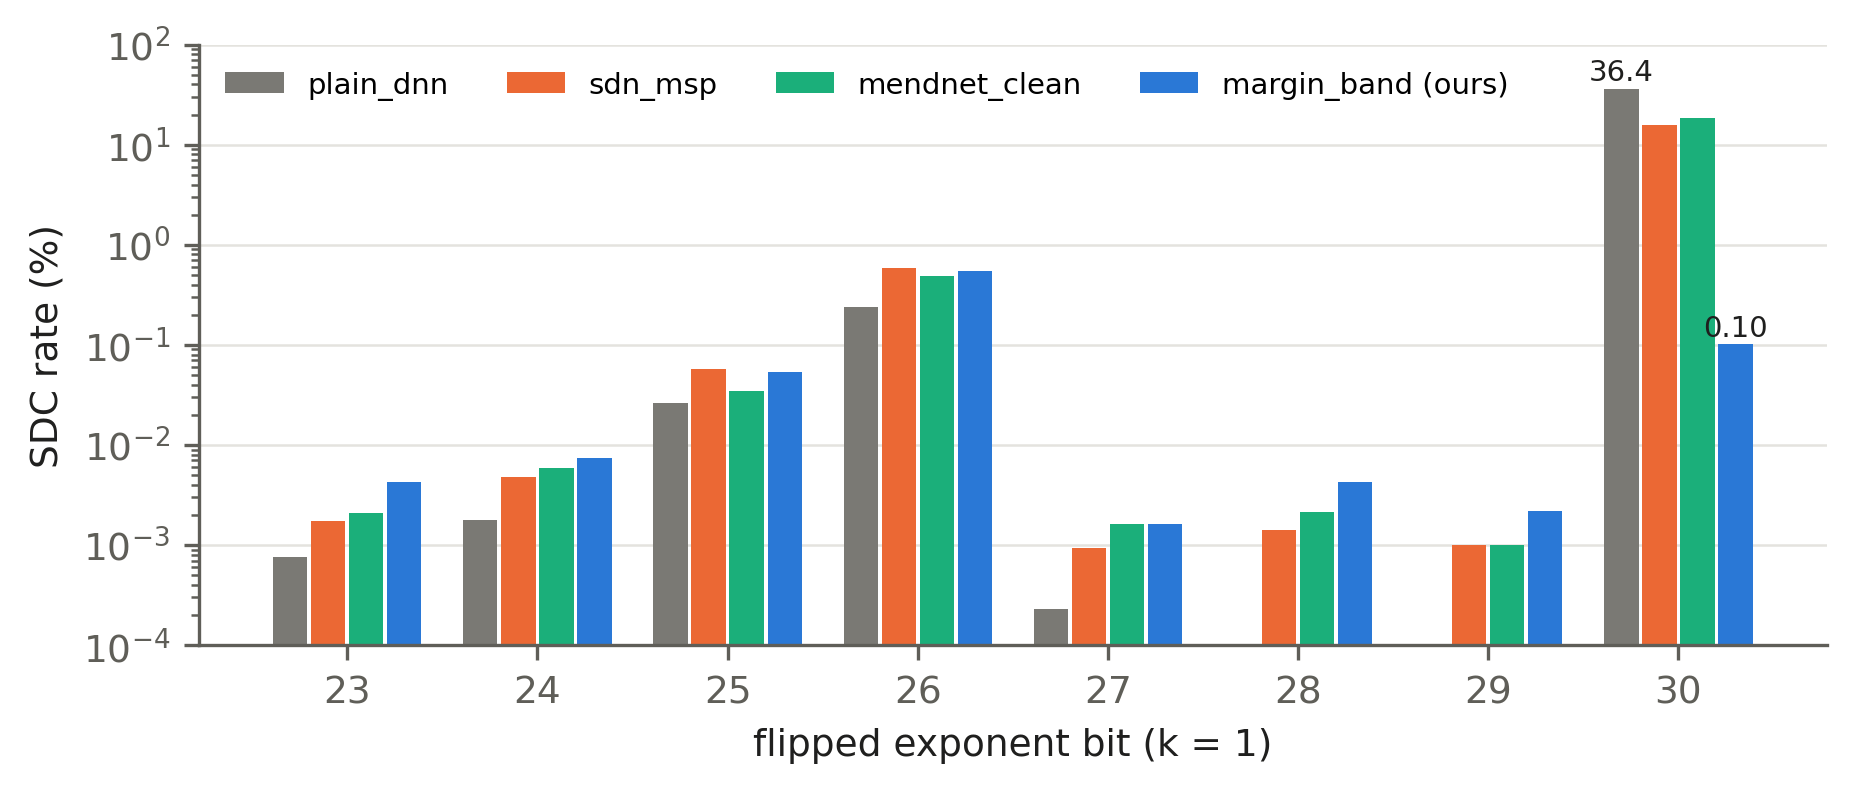
\includegraphics[width=0.95\linewidth]{per_bit.png}
\caption{Per-bit SDC for one faulty weight (log scale; zero bars omitted). Bit 30 dominates the damage of every
unprotected method; the band reduces it by $\approx 150$--$360\times$.}
\label{fig:bit}
\end{figure}

Bit 30 causes almost all the damage (Table~\ref{tab:bit}, Fig.~\ref{fig:bit}): a single flip silently
corrupts $36.4\,\%$ of the plain network's correct answers and $18.5\,\%$ of MENDNet's, but only
$0.10\,\%$ with the band. Bits 27--29 are usually 1 in typical weights, so their flips shrink the weight, which the network
tolerates. The residual SDC of the band comes mostly from bit 26 (a factor of $2^{8}$); for this bit all
methods are similar ($0.24$--$0.67\,\%$), which suggests that such moderate changes keep the logits
inside their clean range.

\subsection{Ablation: which side of the band}\label{sec:ablation}

\begin{table}[H]
\centering\small
\caption{Ablation on the NAS model (exits 16/22/23), \ours, $\alpha=1\,\%$. M0 = same exits and margin
thresholds, no band and no final gate. Slack = accuracy slack of the margin calibration (default $0.5$).}
\label{tab:ablation}
\begin{adjustbox}{max width=\linewidth}
\begin{tabular}{@{}lrrrrrrr@{}}
\toprule
Variant & Clean acc. & FAR & Saved & SDC & Flag & Det.\ ratio & TPR \\
\midrule
M0, unprotected            & 91.9 & 0    & 53.7 & 7.95  & 0      & 0     & 0    \\
band: none                 & 91.9 & 0    & 53.7 & 7.95  & 0      & 0     & 0    \\
band: lower side only      & 91.8 & 0.43 & 53.6 & 7.93  & 0.012  & 0.15  & 4.8  \\
band: upper side only      & 91.4 & 0.55 & 53.6 & 0.194 & 6.28   & 97.0  & 93.7 \\
band: both (\ours)         & 91.3 & 0.98 & 53.6 & 0.143 & 6.33   & 97.8  & 96.3 \\
\midrule
slack 0                    & 91.6 & 0.94 & 36.9 & 0.107 & 9.87   & 98.9  & 90.8 \\
slack 1                    & 91.0 & 1.00 & 55.9 & 0.163 & 6.02   & 97.4  & 97.8 \\
\bottomrule
\end{tabular}
\end{adjustbox}
\end{table}

Table~\ref{tab:ablation} isolates the mechanism. A lower bound alone behaves like no band at all
(SDC $7.93\,\%$ against $7.95\,\%$). The upper bound alone removes $97.6\,\%$ of the SDCs. Adding the lower
side on top of the upper side lowers SDC a little further ($0.194\to0.143\,\%$) at the cost of a higher FAR. The calibration slack trades FLOP saving against SDC: a stricter exit (slack 0) sends
more inputs to the final band and lowers SDC further, but saves only $36.9\,\%$.

\subsection{False-alarm budget}

\begin{table}[H]
\centering\small
\setlength{\tabcolsep}{4pt}
\caption{Sweep of the clean false-alarm budget $\alpha$ (final model, exponent faults).
Columns: measured clean FAR, clean accuracy, SDC rate, run-level TPR (all \%).}
\label{tab:alpha}
\begin{adjustbox}{max width=\linewidth}
\begin{tabular}{@{}lr rrrr rrrr rrrr@{}}
\toprule
 & & \multicolumn{4}{c}{\ours} & \multicolumn{4}{c}{\meth{energy\_band}} & \multicolumn{4}{c}{\meth{mendnet\_clean}} \\
\cmidrule(lr){3-6}\cmidrule(lr){7-10}\cmidrule(l){11-14}
 & $\alpha$ & FAR & Acc & SDC & TPR & FAR & Acc & SDC & TPR & FAR & Acc & SDC & TPR \\
\midrule
 & 0.25 & 0.28 & 91.6 & 0.233 & 90.9 & 0.40 & 91.1 & 0.188 & 82.9 & 0.36 & 91.8 & 7.02 & 2.6 \\
 & 0.5  & 0.43 & 91.5 & 0.231 & 92.8 & 0.55 & 91.0 & 0.187 & 83.8 & 0.52 & 91.7 & 7.13 & 4.9 \\
 & 1    & 0.95 & 91.2 & 0.223 & 93.1 & 0.96 & 90.8 & 0.181 & 85.6 & 1.12 & 91.6 & 7.35 & 4.8 \\
 & 2    & 1.77 & 90.7 & 0.210 & 93.8 & 2.00 & 90.2 & 0.173 & 94.4 & 2.14 & 91.2 & 7.69 & 5.0 \\
 & 5    & 4.85 & 89.0 & 0.140 & 70.5 & 5.03 & 88.4 & 0.146 & 94.3 & 5.42 & 89.8 & 8.47 & 4.5 \\
 & 10   & 5.29 & 88.8 & 0.132 & 69.4 & 9.53 & 85.9 & 0.104 & 69.6 & 10.6 & 86.5 & 11.0 & 5.6 \\
\bottomrule
\end{tabular}
\end{adjustbox}
\end{table}

\begin{figure}[H]
\centering
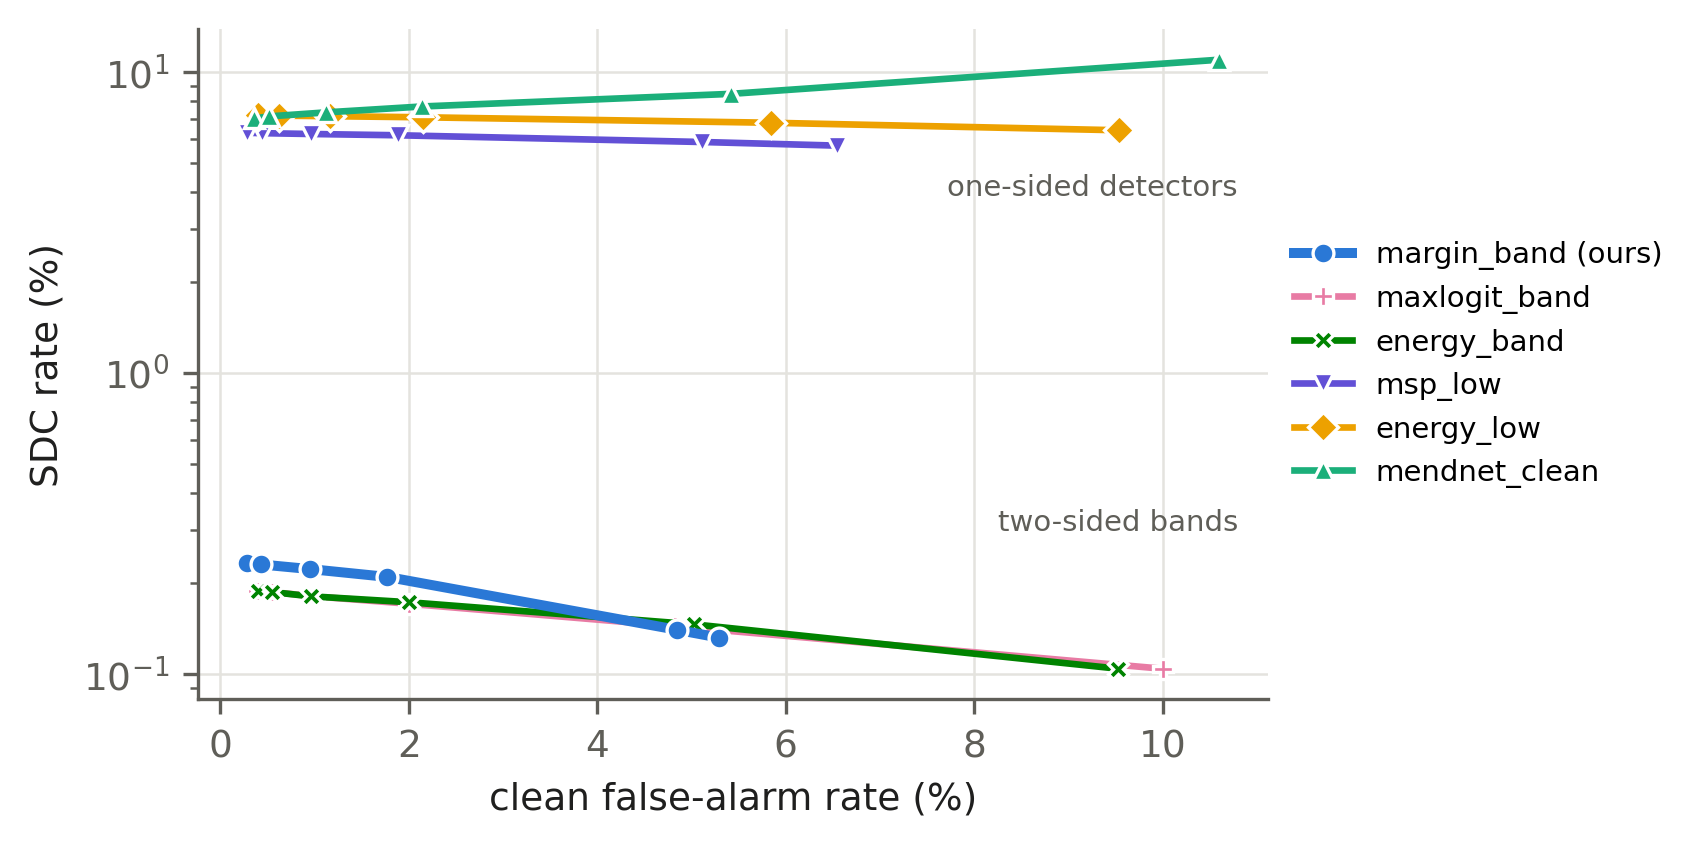
\includegraphics[width=0.75\linewidth]{alpha_sweep.png}
\caption{SDC rate against clean false-alarm rate, $\alpha\in\{0.25,0.5,1,2,5,10\}\,\%$. \meth{maxlogit\_band}
and \meth{energy\_band} nearly coincide. Two-sided bands stay $30$--$70\times$ below one-sided detectors at every budget; raising the budget barely
helps the one-sided detectors.}
\label{fig:alpha}
\end{figure}

Table~\ref{tab:alpha} and Fig.~\ref{fig:alpha} show that the band works already at $\alpha=0.25\,\%$
(SDC $0.233\,\%$, TPR $90.9\,\%$). One-sided detectors gain almost nothing from a larger budget, because the
faulty inputs are not in the low tail they inspect; MENDNet's SDC even rises with the budget. At $\alpha\ge5\,\%$ the run-level TPR of \ours\ drops, most
likely because the binomial test then compares against a higher clean FAR. We use $\alpha=1\,\%$.

\subsection{Other fault models}

\paragraph{INT8 weights.} Table~\ref{tab:int8}: with simulated weight-only INT8, a flipped bit changes a
weight by at most 128 quantisation steps, i.e.\ about the largest weight magnitude of its tensor, so faults are almost harmless for every method
(SDC $\le 0.02\,\%$). The band adds little here; this confirms that the threat our method addresses is
specific to floating-point exponents. MENDNet tuned on faulty validation data over-flags in this setting
(FAR $17.8\,\%$).

\begin{table}[H]
\centering\small
\caption{INT8 weight faults (simulated weight-only INT8, one bit of $k$ codes, $k=1..8$, final model).}
\label{tab:int8}
\begin{adjustbox}{max width=\linewidth}
\begin{tabular}{@{}lrrrrrr@{}}
\toprule
Method & Clean acc. & FAR & SDC & Flag & Det.\ ratio & Acc.\ / fallback \\
\midrule
\meth{plain\_dnn}          & 92.3 & 0    & 0.0086  & 0       & 0    & 92.3 / 92.3 \\
\meth{sdn\_msp}            & 91.7 & 0    & 0.0188  & 0       & 0    & 91.7 / 91.7 \\
\meth{msp\_low}            & 91.3 & 1.06 & 0.0127  & 0.0059  & 31.8 & 91.3 / 91.7 \\
\meth{energy\_low}         & 91.1 & 1.21 & 0.0127  & 0.0013  & 9.1  & 91.1 / 91.6 \\
\meth{mendnet\_clean}      & 91.5 & 1.16 & 0.0203  & 0.0020  & 9.2  & 91.5 / 91.9 \\
\meth{mendnet\_faulty\_val}& 80.7 & 17.8 & 0.00001 & 0.023   & 100  & 80.7 / 92.3 \\
\midrule
\ours\ (\textbf{ours})     & 91.2 & 0.97 & 0.0200  & 0.0060  & 23.1 & 91.2 / 91.7 \\
\meth{maxlogit\_band}      & 90.8 & 1.17 & 0.0171  & 0.0099  & 36.6 & 90.8 / 91.4 \\
\meth{energy\_band}        & 90.7 & 1.16 & 0.0118  & 0.0033  & 21.9 & 90.7 / 91.3 \\
\meth{margin\_multiband}   & 91.3 & 0.95 & 0.0162  & 0.0071  & 30.5 & 91.3 / 91.8 \\
\meth{margin\_band\_agree} & 91.4 & 1.13 & 0.0107  & 0.0074  & 40.7 & 91.4 / 92.0 \\
\bottomrule
\end{tabular}
\end{adjustbox}
\end{table}

\paragraph{MENDNet's fault model.} Tables~\ref{tab:mendacc} and~\ref{tab:mendsdc} use MENDNet's own
sign-flip model. The picture is mixed, and we report it as such. When the final classifier is hit (FP1),
the band is the best detector (SDC $0$ at FR $30$--$50\,\%$, while the plain network collapses to
$13.2\,\%$ accuracy at FR $50\,\%$), and fallback restores $91.3\,\%$ accuracy. When an exit head or the
layer right after exit 1 is hit (FP2, FP3), sign flips shrink or scramble the logits rather than inflate
them, the band catches less, and MENDNet tuned on faulty data is often better. When the first convolution
is hit (FP4), every exit sees corrupted features and every method fails.

\begin{table}[H]
\centering\small
\caption{MENDNet fault model (sign flips of FR\,\% of one group's weights): accuracy with fallback (\%).}
\label{tab:mendacc}
\begin{adjustbox}{max width=\linewidth}
\begin{tabular}{@{}llrrrrrr@{}}
\toprule
Group & FR & \meth{plain} & \meth{sdn\_msp} & \meth{mendnet\_clean} & \meth{mendnet\_faulty} & \meth{energy\_band} & \ours \\
\midrule
FP1 final classifier & 10 & 92.2 & 91.7 & 91.8 & 91.2 & 91.2 & 91.6 \\
                     & 30 & 89.9 & 91.5 & 91.6 & 91.0 & 91.0 & 91.3 \\
                     & 50 & 13.2 & 88.8 & 91.3 & 89.7 & 90.7 & 91.3 \\
FP2 exit-2 head      & 10 & 92.3 & 89.8 & 91.6 & 90.2 & 90.3 & 88.8 \\
                     & 30 & 92.3 & 85.5 & 86.2 & 86.8 & 77.9 & 83.7 \\
                     & 50 & 92.3 & 79.7 & 78.8 & 83.1 & 55.0 & 78.3 \\
FP3 first conv after exit 1 & 10 & 90.3 & 88.6 & 89.7 & 88.7 & 89.2 & 88.3 \\
                     & 30 & 24.4 & 70.9 & 64.3 & 75.2 & 63.0 & 71.8 \\
                     & 50 & 10.1 & 67.2 & 64.0 & 71.4 & 63.7 & 72.0 \\
FP4 first conv       & 10 & 85.8 & 84.1 & 85.2 & 83.7 & 84.9 & 83.8 \\
                     & 30 & 41.5 & 40.2 & 41.2 & 39.6 & 41.2 & 38.9 \\
                     & 50 & 16.3 & 16.2 & 16.2 & 15.6 & 16.2 & 15.8 \\
\bottomrule
\end{tabular}
\end{adjustbox}
\end{table}

\begin{table}[H]
\centering\small
\caption{MENDNet fault model: SDC rate (\%) on each method's clean-correct subset.}
\label{tab:mendsdc}
\begin{adjustbox}{max width=\linewidth}
\begin{tabular}{@{}llrrrrrr@{}}
\toprule
Group & FR & \meth{plain} & \meth{sdn\_msp} & \meth{mendnet\_clean} & \meth{mendnet\_faulty} & \meth{energy\_band} & \ours \\
\midrule
FP1 & 10 & 0.47 & 0.23 & 0.10 & 0.16 & 0.015 & 0.003 \\
    & 30 & 3.61 & 0.78 & 0.14 & 0.50 & 0     & 0 \\
    & 50 & 86.7 & 3.55 & 0.14 & 1.89 & 0     & 0 \\
FP2 & 10 & 0    & 3.35 & 0.89 & 2.06 & 1.98  & 4.47 \\
    & 30 & 0    & 7.73 & 6.49 & 5.52 & 15.3  & 9.65 \\
    & 50 & 0    & 14.0 & 14.6 & 9.56 & 40.2  & 15.4 \\
FP3 & 10 & 3.86 & 5.23 & 3.44 & 4.35 & 3.82  & 5.08 \\
    & 30 & 75.6 & 24.2 & 20.4 & 18.9 & 25.5  & 20.4 \\
    & 50 & 90.4 & 27.7 & 7.44 & 22.6 & 8.5   & 13.8 \\
FP4 & 10 & 9.07 & 10.7 & 8.10 & 10.8 & 8.8   & 9.85 \\
    & 30 & 57.0 & 58.3 & 37.4 & 58.8 & 43.0  & 47.4 \\
    & 50 & 84.0 & 84.1 & 43.2 & 84.6 & 53.4  & 61.9 \\
\bottomrule
\end{tabular}
\end{adjustbox}
\end{table}

\subsection{Choice of exits and robustness}

\begin{table}[H]
\centering\small
\setlength{\tabcolsep}{3.5pt}
\caption{Different exit configurations, \ours, $\alpha=1\,\%$, exponent faults. \meth{old1623}: hand-placed exits
16/23; \meth{nas}: best TPE trial with proxy heads; \meth{final}: selected after full training;
\meth{p3}: lowest head-fault SDC from the fault-aware search; \meth{p4}: lowest FLOPs with exactly 2 exits.}
\label{tab:models}
\begin{adjustbox}{max width=\linewidth}
\begin{tabular}{@{}llrrrrrrrrrr@{}}
\toprule
Model & Exits & Head params & Clean acc. & FAR & Saved & SDC G1 & SDC G2 & SDC G3 & SDC HEADS & SDC all & Flag all \\
\midrule
\meth{old1623} & 16, 23     & 1{,}102{,}100 & 91.2 & 0.92 & 52.5 & 0.381 & 0.076 & 0.0040 & 0.020 & 0.120 & 7.20 \\
\meth{nas}     & 16, 22, 23 & 411{,}614     & 91.3 & 0.98 & 53.6 & 0.420 & 0.068 & 0.0032 & 0.083 & 0.143 & 6.33 \\
\meth{final}   & 13, 16, 26 & 260{,}830     & 91.2 & 0.95 & \textbf{60.5} & 0.621 & 0.089 & 0.0019 & 0.179 & 0.223 & 5.25 \\
\meth{p3}      & 13, 19, 26 & 1{,}239{,}742 & 91.2 & 1.13 & 59.3 & 0.549 & 0.061 & 0.0025 & 0.050 & 0.166 & 5.57 \\
\meth{p4}      & 12, 19     & 329{,}108     & 90.8 & 1.28 & 59.3 & 0.641 & 0.086 & 0.0018 & 0.135 & 0.216 & 5.21 \\
\bottomrule
\end{tabular}
\end{adjustbox}
\end{table}

All configurations (Table~\ref{tab:models}) reach SDC between $0.12$ and $0.22\,\%$, so the detection
mechanism does not depend on a particular exit placement. Earlier first exits save more compute but leave a
smaller G1 and more inputs exposed in the heads, which slightly raises SDC: the selected model trades
$0.1$ points of SDC for $8$ points of FLOP saving compared with the hand-placed 16/23 model, with $4\times$
fewer head parameters.

\begin{table}[H]
\centering\small
\caption{Head-training seeds (final configuration, seeds 42, 1, 2), mean $\pm$ std. Seed 42 uses 100 runs per
setting, seeds 1 and 2 use 20.}
\label{tab:seeds}
\begin{adjustbox}{max width=\linewidth}
\begin{tabular}{@{}lrrrrr@{}}
\toprule
Method & Clean acc. & FAR & Saved & SDC & Flag \\
\midrule
\ours\              & $91.1\pm0.22$ & $1.07\pm0.11$ & $57.1\pm3.0$ & $0.211\pm0.011$ & $5.50\pm0.27$ \\
\meth{energy\_band} & $90.9\pm0.25$ & $0.96\pm0.01$ & $54.9\pm1.0$ & $0.199\pm0.030$ & $5.47\pm0.39$ \\
\meth{mendnet\_clean} & $91.5\pm0.09$ & $1.03\pm0.08$ & $55.0\pm0.8$ & $6.66\pm0.59$ & $0.028\pm0.002$ \\
\bottomrule
\end{tabular}
\end{adjustbox}
\end{table}

Retraining the heads with different seeds (Table~\ref{tab:seeds}) changes the SDC rate of \ours\ by only
$\pm0.011$ points.

\subsection{Latency}

\begin{table}[H]
\centering\small
\caption{Batch-1 latency (ms) with real early stopping, \ours, $\alpha=1\,\%$. \emph{plain}: backbone only;
\emph{all exits}: every head computed, no stopping; \emph{early stop}: inference stops at the accepting exit.
CPU: 8 threads, 500 images; GPU: A100-SXM4-40GB, 2{,}000 images. Predictions and exits of the early-stop run
agree with the offline evaluation on $99.8$--$100\,\%$ of the images.}
\label{tab:latency}
\begin{adjustbox}{max width=\linewidth}
\begin{tabular}{@{}l rrrr rrrr@{}}
\toprule
 & \multicolumn{4}{c}{CPU} & \multicolumn{4}{c}{GPU} \\
\cmidrule(lr){2-5}\cmidrule(l){6-9}
Model & plain & all exits & early stop & speed-up & plain & all exits & early stop & speed-up \\
\midrule
\meth{old1623} & 10.3 & 11.4 & 4.25 & 2.43$\times$ & 1.90 & 2.52 & 1.38 & 1.37$\times$ \\
\meth{nas}     & 10.4 & 12.1 & 4.11 & 2.52$\times$ & 1.93 & 3.14 & 1.48 & 1.31$\times$ \\
\meth{final}   & 11.4 & 12.5 & 3.42 & \textbf{3.32}$\times$ & 1.91 & 3.03 & 1.37 & 1.39$\times$ \\
\meth{p3}      & 10.3 & 12.2 & 3.34 & 3.10$\times$ & 1.91 & 2.94 & 1.28 & 1.49$\times$ \\
\meth{p4}      & 10.3 & 12.1 & 3.35 & 3.07$\times$ & 1.91 & 2.73 & 1.24 & 1.54$\times$ \\
\bottomrule
\end{tabular}
\end{adjustbox}
\end{table}

\begin{figure}[H]
\centering
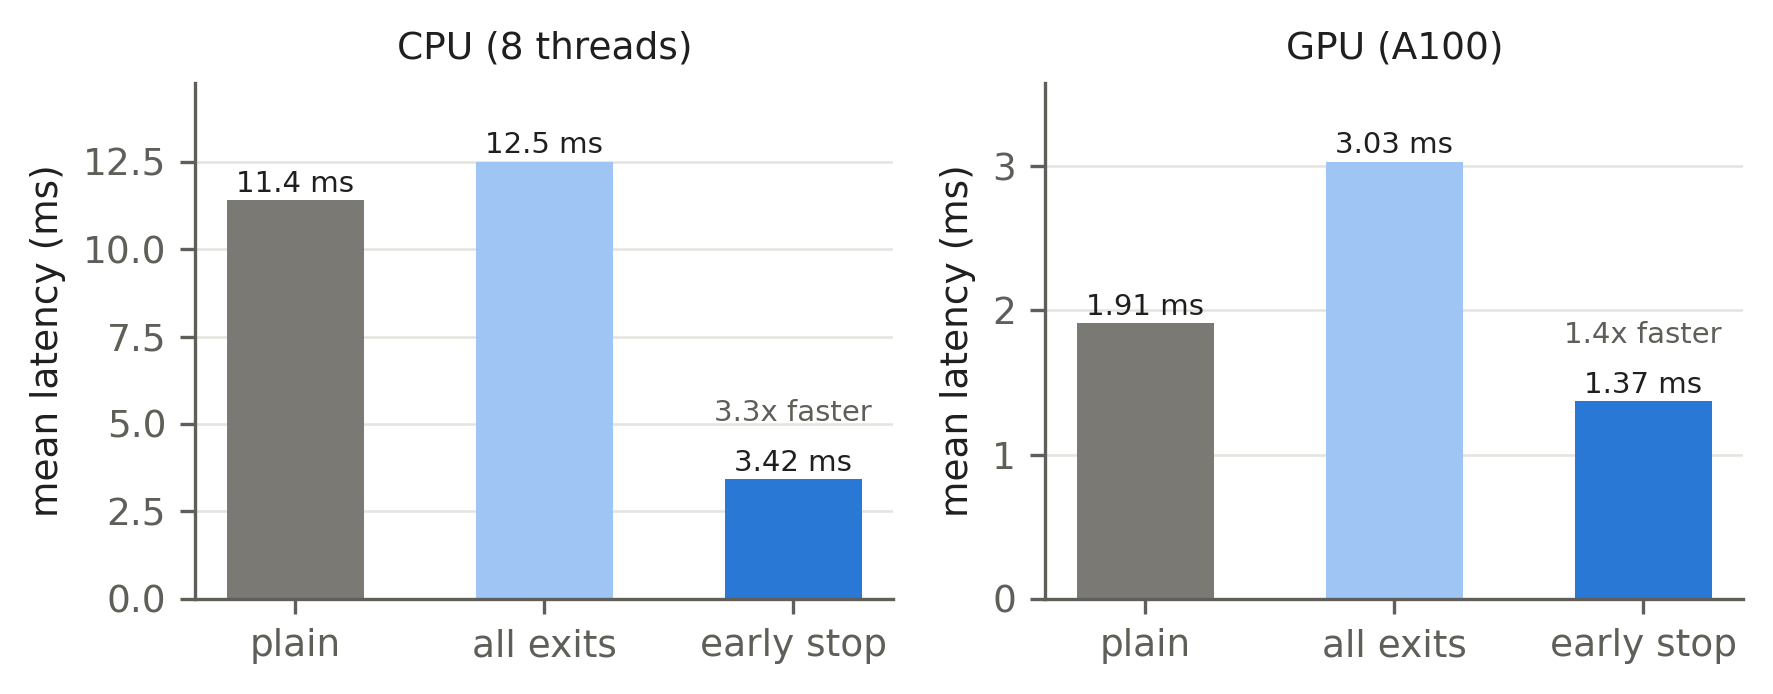
\includegraphics[width=0.85\linewidth]{latency.png}
\caption{Batch-1 latency of the final model. Early stopping turns the $60.5\,\%$ FLOP saving into a $3.3\times$
CPU and $1.4\times$ GPU speed-up; computing all exits without stopping is slower than the plain network.}
\label{fig:latency}
\end{figure}

Real early stopping (Table~\ref{tab:latency}, Fig.~\ref{fig:latency}) gives a $3.3\times$ speed-up on CPU. On
the GPU, batch-1 inference of a small CIFAR network does not saturate the device, so the gain is
$1.4\times$. Computing every exit without stopping costs $9\,\%$ (CPU) to $59\,\%$ (GPU) extra time; the
detector should therefore be deployed together with early stopping, not as an add-on to a full forward pass.

\subsection{Hardware cost}

\begin{table}[H]
\centering\small
\caption{Operations per exit decision of each rule.}
\label{tab:ops}
\begin{adjustbox}{max width=\linewidth}
\begin{tabular}{@{}ll@{}}
\toprule
Rule & Operations per decision \\
\midrule
\meth{plain\_dnn}           & none (no exits) \\
\meth{sdn\_msp}, \meth{msp\_low} & softmax (10 exp, division), max \\
\meth{energy\_low}          & exp, log (log-sum-exp) \\
\meth{mendnet}              & softmax (exp, division), max, log-sum-exp (exp, log) \\
\meth{energy\_band}         & exp, log + comparators \\
\meth{maxlogit\_band}       & comparators \\
\ours                       & top-2 comparator tree, 1 subtraction, 3 comparators \\
\meth{margin\_multiband}    & comparators, 1 subtraction, 9 additions \\
\meth{margin\_band\_agree}  & comparators, 1 subtraction (+ next exit computed) \\
\bottomrule
\end{tabular}
\end{adjustbox}
\end{table}

\begin{table}[H]
\centering\small
\caption{Theoretical hardware cost of the exits (HLS synthesis is future work).}
\label{tab:hw}
\begin{adjustbox}{max width=\linewidth}
\begin{tabular}{@{}lrrr@{}}
\toprule
Model & Exits & Head params & Head FLOP overhead (\%) \\
\midrule
\meth{old1623} & 2 & 1{,}102{,}100 & 0.68 \\
\meth{nas}     & 3 & 411{,}614     & 2.10 \\
\meth{final}   & 3 & 260{,}830     & 3.67 \\
\meth{p3}      & 3 & 1{,}239{,}742 & 2.12 \\
\meth{p4}      & 2 & 329{,}108     & 4.58 \\
\bottomrule
\end{tabular}
\end{adjustbox}
\end{table}

The decision logic of \ours\ (Table~\ref{tab:ops}) is a top-2 search over 10 logits, one subtraction and
three comparisons ($m\ge t$, $M\ge L$, $M\le U$) per exit, plus two comparisons at the final classifier.
It needs no exponential, logarithm or divider, unlike softmax-, entropy- or energy-based rules and MENDNet.
The heads of the final model add $3.67\,\%$ FLOPs to a full pass (Table~\ref{tab:hw}), which is paid only by
inputs that reach all exits.

\subsection{Exit-placement search}\label{sec:nasres}

Every step of the exit search was checked by its own comparison:
\begin{enumerate}
  \setcounter{enumi}{-1}
  \item \textbf{Search strategy and search space:} TPE vs NSGA-II vs random search, restricted spaces, fixed rules
        and fault-aware objectives (Table~\ref{tab:nas}).
  \item \textbf{Proxy training:} short proxy training vs full training of the heads (Table~\ref{tab:proxy}).
  \item \textbf{Fault probe:} the cheap fault probe of the fault-aware search vs a full fault campaign.
  \item \textbf{Searched vs hand-placed designs} under the same scoring (Table~\ref{tab:picks}).
  \item \textbf{Fault behaviour of the searched model} vs the hand-placed model, with statistical tests
        (Table~\ref{tab:paired}).
  \item \textbf{Full training of the top candidates} and the final pick (Table~\ref{tab:top5}).
\end{enumerate}

\paragraph{Step 0: search strategy and search space.}

\begin{table}[H]
\centering\small
\setlength{\tabcolsep}{4pt}
\caption{Search variants: hypervolume (HV) on a common reference point (accuracy, expected FLOPs, head
parameters), 3 sampler seeds (1 for D1/D2). Best feasible = lowest expected MFLOPs with accuracy
$\ge$ backbone $-1$.}
\label{tab:nas}
\begin{adjustbox}{max width=\linewidth}
\begin{tabular}{@{}lllrrrr@{}}
\toprule
Variant & Sampler & Search space / objectives & HV (mean $\pm$ std) & Pareto pts & Best feasible MFLOPs & Wall (min) \\
\midrule
A1 & TPE       & full space                      & $\mathbf{7.04\pm0.45}$ & 63.3 & 315 & 10.5 \\
A2 & NSGA-II   & full space (pop.\ 50)           & $6.25\pm0.14$ & 33.7 & 321 & 7.6 \\
A3 & random    & full space                      & $6.23\pm0.28$ & 36.3 & 318 & 11.8 \\
B1 & TPE       & fixed menu heads A1--A5         & $6.18\pm0.17$ & 72.0 & 335 & 0.9 \\
B2 & TPE       & positions only (default head)   & $5.14\pm0.10$ & 103  & 327 & 0.1 \\
B3 & TPE       & heads only (positions 16, 23)   & $6.77\pm0.20$ & 68.3 & 306 & 0.2 \\
C1 & TPE       & exactly 1 exit                  & $6.01\pm0.01$ & 63.0 & 342 & 1.0 \\
C2 & TPE       & exactly 2 exits                 & $6.76\pm0.63$ & 57.3 & 314 & 2.1 \\
C3 & TPE       & exactly 3 exits                 & $6.88\pm0.38$ & 33.7 & 308 & 1.6 \\
D1 & TPE       & rule fixed: \ours               & $6.25$        & 54.0 & 324 & 1.1 \\
D2 & TPE       & rule fixed: \meth{maxlogit\_band} & $6.60$      & 69.0 & 328 & 0.7 \\
E1 & TPE       & + head-fault SDC (4 objectives) & $6.68\pm0.27$ & 54.0 & 310 & 19.0 \\
E2 & TPE       & acc., FLOPs, exposure           & $7.00\pm0.23$ & 34.7 & 298 & 19.1 \\
\bottomrule
\end{tabular}
\end{adjustbox}
\end{table}

TPE over the full space reaches the highest hypervolume (Table~\ref{tab:nas}), clearly above NSGA-II and
random search with the same budget. Searching both positions and heads matters: positions alone (B2) are the
worst variant, and a fixed menu of heads (B1) is also worse. Allowing up to three exits beats a single exit.
Adding fault-related objectives (E1, E2) does not raise the common hypervolume, which supports our design of
keeping fault detection in the calibrated rule rather than in the search.

\paragraph{Step 1: is the 8-epoch proxy trustworthy?} Every trial trains its heads for only 8 epochs on cached
features. Table~\ref{tab:proxy} compares proxy accuracy with full 60-epoch training on 20 random head
configurations. The proxy underestimates accuracy by about 3 points but ranks the heads almost exactly like full
training (Spearman $\rho=0.987$). An earlier check on 5 heads gave $\rho=0.90$ ($p=0.037$). A 16-epoch proxy ranks
only marginally better, so 8 epochs were kept.

\begin{table}[H]
\centering\small
\caption{Proxy fidelity: head validation accuracy after a short proxy training vs full training (60 epochs),
20 random configurations.}
\label{tab:proxy}
\begin{adjustbox}{max width=\linewidth}
\begin{tabular}{@{}lrrrr@{}}
\toprule
Proxy & Spearman $\rho$ & $p$ & Kendall $\tau$ & Mean gap to full training (points) \\
\midrule
4 epochs           & 0.988 & $5\cdot10^{-16}$ & 0.926 & 4.27 \\
\textbf{8 epochs (used)} & \textbf{0.987} & $1\cdot10^{-15}$ & \textbf{0.934} & 3.07 \\
16 epochs          & 0.995 & $2\cdot10^{-19}$ & 0.966 & 2.40 \\
\bottomrule
\end{tabular}
\end{adjustbox}
\end{table}

\paragraph{Step 2: is the fault probe of the fault-aware search trustworthy?} Variant E1 adds a fourth objective,
the SDC caused by 40 random head faults (a probe). On 10 configurations the probe ranks the heads like a full
200-fault campaign (Spearman $\rho=0.875$, $p=9\cdot10^{-4}$, Kendall $\tau=0.72$), so E1 optimises a meaningful
quantity; it still does not improve the common hypervolume (Table~\ref{tab:nas}).

\paragraph{Step 3: searched designs vs hand-placed designs.} Table~\ref{tab:picks} scores the picks of the search
variants and two hand-placed designs with the same procedure (proxy heads, VAL\_SEL, $\alpha=1\,\%$). Every searched
design saves more computation than the hand-placed ones (50--51\,\% against 40--46\,\%) with $3$--$4.5\times$ fewer
head parameters than the hand-placed 6/13/23 design. The lowest-parameter pick (P2, a single tiny exit at
module 2) saves almost nothing; this is why the final pick rule minimises FLOPs, not parameters.

\begin{table}[H]
\centering\small
\setlength{\tabcolsep}{4pt}
\caption{Picks of the search variants vs hand-placed designs (proxy heads, VAL\_SEL, \ours, $\alpha=1\,\%$).
Head-fault SDC = probe SDC (\%) for faults in the heads.}
\label{tab:picks}
\begin{adjustbox}{max width=\linewidth}
\begin{tabular}{@{}llllrrrrr@{}}
\toprule
Design & Source & Exits & & Acc. & Acc.\ deployed & Saved & Head params & Head-fault SDC \\
\midrule
hand-placed 6/13/23 & default heads (A3)           & 6, 13, 23   & & 92.52 & 91.52 & 46.4 & 1{,}843{,}486 & 0.014 \\
hand-placed 16/23   & menu heads A4, A3            & 16, 23      & & 92.76 & 91.72 & 39.8 & 1{,}102{,}100 & 0.001 \\
\midrule
P1 (= \meth{nas})   & A1 TPE, lowest FLOPs         & 16, 22, 23  & & 92.36 & 91.80 & 50.3 & 411{,}614     & 0.011 \\
P2                  & A1 TPE, fewest head params   & 2           & & 92.60 & 91.76 & 0.6  & 650           & 0.320 \\
P3 (= \meth{p3})    & E1, lowest head-fault SDC    & 13, 19, 26  & & 92.32 & 91.60 & 50.6 & 1{,}239{,}742 & 0     \\
P4 (= \meth{p4})    & C2 (2 exits), lowest FLOPs   & 12, 19      & & 92.48 & 91.80 & 51.1 & 329{,}108     & 0.035 \\
\bottomrule
\end{tabular}
\end{adjustbox}
\end{table}

\paragraph{Step 4: does the searched model change fault behaviour?} Table~\ref{tab:paired} compares the NAS model
(16/22/23) with the hand-placed 16/23 model under identical faults (paired tests, Holm correction). The
differences are statistically significant but small in absolute terms (hundredths of a percentage point of SDC):
the search mainly buys compute and head size, while the protection comes from the band. Faults in the NAS heads
cause more SDC ($0.083$ vs $0.020\,\%$) because its heads are smaller and accept more images.

\begin{table}[H]
\centering\small
\caption{NAS model vs hand-placed 16/23 model, \ours, exponent faults, 800 runs per location. G1--G3: Wilcoxon
signed-rank paired by identical faults; HEADS: Mann-Whitney U. $p$ after Holm correction.}
\label{tab:paired}
\begin{adjustbox}{max width=\linewidth}
\begin{tabular}{@{}lrrrrrr@{}}
\toprule
 & \multicolumn{3}{c}{SDC rate (\%)} & \multicolumn{3}{c}{Flag rate (\%)} \\
\cmidrule(lr){2-4}\cmidrule(l){5-7}
Location & 16/23 & NAS & $p_{\mathrm{Holm}}$ & 16/23 & NAS & $p_{\mathrm{Holm}}$ \\
\midrule
G1    & 0.380  & 0.420  & $3\cdot10^{-14}$ & 22.31 & 20.70 & $9\cdot10^{-5}$ \\
G2    & 0.076  & 0.068  & $3\cdot10^{-19}$ & 4.50  & 2.96  & $2\cdot10^{-17}$ \\
G3    & 0.0039 & 0.0032 & $6\cdot10^{-6}$  & 1.48  & 1.36  & $1\cdot10^{-48}$ \\
HEADS & 0.020  & 0.083  & $1\cdot10^{-12}$ & 0.63  & 0.30  & 0.17 (n.s.) \\
\bottomrule
\end{tabular}
\end{adjustbox}
\end{table}

\paragraph{Step 5: full training of the top candidates.}

\begin{table}[H]
\centering\small
\setlength{\tabcolsep}{4pt}
\caption{Top candidates after full training, scored on VAL\_SEL (\%); ``deployed'' includes the final band
($\alpha=1\,\%$). The pick rule selects \meth{s11\_t229} (lowest expected FLOPs with accuracy $\ge91.84\,\%$).}
\label{tab:top5}
\begin{adjustbox}{max width=\linewidth}
\begin{tabular}{@{}llllrrrrl@{}}
\toprule
Candidate & Exits & Rule & & Acc. & Acc.\ deployed & Saved & Head params & Head val acc.\ (full training) \\
\midrule
\meth{s1\_t94} (\meth{nas}) & 16, 22, 23 & margin  & & 92.3 & 91.2 & 54.0 & 411{,}614 & 89.4 / 91.0 / 92.0 \\
\meth{s21\_t81}             & 12, 16, 22 & margin  & & 93.0 & 92.2 & 45.8 & 166{,}814 & 84.4 / 89.8 / 91.4 \\
\meth{s21\_t198}            & 16, 19     & margin  & & 91.9 & 90.8 & 52.7 & 65{,}652  & 88.0 / 90.0 \\
\textbf{\meth{s11\_t229}} (\meth{final}) & 13, 16, 26 & margin & & 92.0 & 91.2 & \textbf{60.8} & 260{,}830 & 86.6 / 90.4 / 91.6 \\
\meth{s11\_t32}             & 16, 26     & maxlogit & & 92.6 & 91.8 & 44.5 & 139{,}092 & 89.4 / 92.1 \\
\meth{s1\_t239}             & 5, 16, 23  & margin  & & 92.2 & 91.2 & 51.5 & 62{,}414  & 57.2 / 88.5 / 90.3 \\
\bottomrule
\end{tabular}
\end{adjustbox}
\end{table}

Full training changes the ranking of the proxy (Table~\ref{tab:top5}): the best proxy trial (\meth{s1\_t94})
saves $54.0\,\%$, while \meth{s11\_t229} saves $60.8\,\%$ at the same accuracy. Re-scoring a few candidates with
fully trained heads is therefore worth its cost.

\subsection{Reproducibility check}

\begin{table}[H]
\centering\small
\caption{Re-evaluation of an earlier, independent campaign from the stored logits (\ours, same calibration,
identical faults).}
\label{tab:repro}
\begin{adjustbox}{max width=\linewidth}
\begin{tabular}{@{}lrrrrr@{}}
\toprule
Model & Runs & Identical faults & Exact SDC/flag match & $|\Delta|$ SDC & Images \\
\midrule
\meth{nas}     & 3{,}200 & 3{,}200 & 3{,}200 & 0 & 29{,}206{,}400 \\
\meth{old1623} & 3{,}200 & 3{,}199 & 3{,}199 & 0 & 29{,}190{,}875 \\
\bottomrule
\end{tabular}
\end{adjustbox}
\end{table}

The logit-storing campaigns reproduce an earlier, independently implemented campaign exactly on every run with
identical faults (Table~\ref{tab:repro}), which validates the offline evaluation used for all comparisons.

% -----------------------------------------------------------------------------------------------------
\section{Discussion and limitations}\label{sec:disc}

\begin{itemize}
  \item \textbf{Detection, not correction.} The band turns silent errors into flagged ones; it does not repair
        the faulty weight. Accuracy with fallback rises only from $86.4$ to $87.4\,\%$. Because harmful fault
        runs are detected within a median of 200 images ($93.1\,\%$ TPR), a system can react by reloading the
        weights and re-running the flagged inputs; evaluating this recovery loop is future work.
  \item \textbf{Fault model scope.} The method targets faults that inflate activations, which are the dominant
        faults in FP32. Under MENDNet's sign-flip model it is not uniformly better (Tables~\ref{tab:mendacc},
        \ref{tab:mendsdc}), and in INT8 the faults are nearly harmless for all methods.
  \item \textbf{Faults before the first exit} cannot be avoided by early exit; the band catches most of them
        through the final classifier (SDC $0.62\,\%$ in G1), but this location remains the main source of
        residual SDC.
  \item \textbf{Scope of evaluation.} One backbone and one dataset (VGG16-BN, CIFAR-10); weight faults only
        (no activation or control faults); INT8 is simulated weight-only quantisation; the hardware cost is
        theoretical until HLS synthesis.
        % TODO: decide whether to add a second backbone / dataset before submission.
\end{itemize}

% -----------------------------------------------------------------------------------------------------
\section{Conclusion}

Early exits can be a fault detector at almost no cost. A two-sided band on the maximum logit, calibrated on
clean data with a $1\,\%$ false-alarm budget, catches the over-confident outputs produced by exponent-bit faults
that confidence-based detectors and MENDNet miss. On VGG16-BN / CIFAR-10 it reduces silent data corruption from
$13.4\,\%$ to $0.22\,\%$, detects $93\,\%$ of harmful fault runs, keeps a $60.5\,\%$ FLOP saving with a
$3.3\times$ CPU speed-up, and needs only comparators and one subtraction per exit.

% -----------------------------------------------------------------------------------------------------
\begin{thebibliography}{99}
\bibitem{branchynet} S.~Teerapittayanon, B.~McDanel, H.~T.~Kung, ``BranchyNet: Fast inference via early exiting
  from deep neural networks,'' in \emph{Proc.\ ICPR}, 2016.
\bibitem{sdn} Y.~Kaya, S.~Hong, T.~Dumitras, ``Shallow-deep networks: Understanding and mitigating network
  overthinking,'' in \emph{Proc.\ ICML}, 2019.
\bibitem{msp} D.~Hendrycks, K.~Gimpel, ``A baseline for detecting misclassified and out-of-distribution examples
  in neural networks,'' in \emph{Proc.\ ICLR}, 2017.
\bibitem{energy} W.~Liu, X.~Wang, J.~Owens, Y.~Li, ``Energy-based out-of-distribution detection,'' in
  \emph{Proc.\ NeurIPS}, 2020.
\bibitem{mendnet} S.~Kundu, M.~Haque, S.~Das, W.~Yang, K.~Basu, ``MENDNet: Just-in-time fault detection and
  mitigation in AI systems with uncertainty quantification and multi-exit networks,'' in \emph{Proc.\ 61st
  ACM/IEEE Design Automation Conference (DAC)}, 2024, pp.~1--6.
\bibitem{ranger} Z.~Chen, G.~Li, K.~Pattabiraman, ``A low-cost fault corrector for deep neural networks through
  range restriction,'' in \emph{Proc.\ DSN}, 2021.
\bibitem{ftclipact} L.-H.~Hoang, M.~A.~Hanif, M.~Shafique, ``FT-ClipAct: Resilience analysis of deep neural
  networks and improving their fault tolerance using clipped activation,'' in \emph{Proc.\ DATE}, 2020.
\bibitem{maxlogit} D.~Hendrycks, S.~Basart, M.~Mazeika, A.~Zou, J.~Kwon, M.~Mostajabi, J.~Steinhardt, D.~Song,
  ``Scaling out-of-distribution detection for real-world settings,'' in \emph{Proc.\ ICML}, 2022.
\bibitem{bigLittle} E.~Park, D.~Kim, S.~Kim, Y.-D.~Kim, G.~Kim, S.~Yoon, S.~Yoo, ``Big/little deep neural network
  for ultra low power inference,'' in \emph{Proc.\ CODES+ISSS}, 2015.
\bibitem{li2017} G.~Li \emph{et al.}, ``Understanding error propagation in deep learning neural network (DNN)
  accelerators and applications,'' in \emph{Proc.\ SC}, 2017.
\bibitem{ares} B.~Reagen \emph{et al.}, ``Ares: A framework for quantifying the resilience of deep neural
  networks,'' in \emph{Proc.\ DAC}, 2018.
\bibitem{optuna} T.~Akiba, S.~Sano, T.~Yanase, T.~Ohta, M.~Koyama, ``Optuna: A next-generation hyperparameter
  optimization framework,'' in \emph{Proc.\ KDD}, 2019.
\bibitem{tpe} J.~Bergstra, R.~Bardenet, Y.~Bengio, B.~K\'egl, ``Algorithms for hyper-parameter optimization,'' in
  \emph{Proc.\ NeurIPS}, 2011.
\bibitem{nsga2} K.~Deb, A.~Pratap, S.~Agarwal, T.~Meyarivan, ``A fast and elitist multiobjective genetic algorithm:
  NSGA-II,'' \emph{IEEE Trans.\ Evol.\ Comput.}, vol.~6, no.~2, pp.~182--197, 2002.
\end{thebibliography}

\end{document}
